\begin{minipage}{\textwidth}
		
		\item Los delfines oceánicos emiten sonidos y luego escuchan la frecuencia del sonido reflejado de su presa. El delfín nada con una rapidez $v_d$ y emite sonidos con frecuencia $f_d$; la frecuencia que oye reflejada de un pez que nada hacia el delfín con rapidez $v_p$ tiene un valor más alto $f_r$.

		\begin{enumerate}
			\item Con estos términos, determine una expresión algebraica para la velocidad del sonido en el agua de mar.
			\item Si $f_d = 80.7$ [kHz], $f_r = 89.6$ [kHz], $v_d= 60$ [km/h] y $v_p=20$ [km/h]. Calcule la velocidad del sonido en el agua de mar.
			\item Compare la velocidad del sonido en el agua de mar con la velocidad del sonido en el aire (340[m/s]). Discuta brevemente su resultado.
		\end{enumerate}
		
\end{minipage}

\textbf{\underline{Solución:}}

\begin{enumerate}
\item
Se tiene el siguiente sistema de referencia inicial:
\begin{figure}[H]
	\centering
	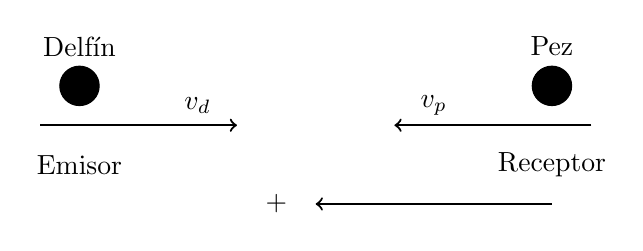
\begin{tikzpicture}
	\filldraw [fill=black] (0,0)circle(.25) (6,0)circle(.25);
	\draw [thick,->] (-.5,-.5)--(2,-.5);
	\draw [thick,->] (6.5,-.5)--(4,-.5);
	\draw [thick,->] (6,-1.5)--(3,-1.5);
	\draw [dotted]
	(0,.5) node {Delfín}
	(6,.5) node {Pez}
	(0,-1) node {Emisor}
	(6,-1) node {Receptor}
	(1.5,-.25) node {\(v_d\)}
	(4.5,-.25) node {\(v_p\)}
	(2.5,-1.5) node {\(+\)}
	;
	\end{tikzpicture}
\end{figure}

luego:
\begin{equation*}
f_{\text{p}}=\frac{v_{\text{s}}+v_{\text{p}}}{v_{\text{s}}-v_{\text{d}}}f_{\text{d}}
\end{equation*}
Y cuando el delfín se convierte en receptor se tiene:

\begin{minipage}{0.6\textwidth}
	\begin{figure}[H]
		\centering
		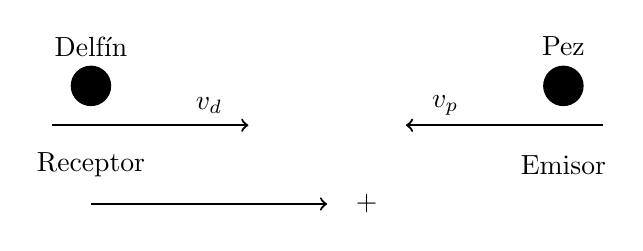
\begin{tikzpicture}
		\filldraw [fill=black] (0,0)circle(.25) (6,0)circle(.25);
		\draw [thick,->] (-.5,-.5)--(2,-.5);
		\draw [thick,->] (6.5,-.5)--(4,-.5);
		\draw [thick,->] (0,-1.5)--(3,-1.5);
		\draw [dotted]
			(0,.5) node {Delfín}
			(6,.5) node {Pez}
			(6,-1) node {Emisor}
			(0,-1) node {Receptor}
			(1.5,-.25) node {\(v_d\)}
			(4.5,-.25) node {\(v_p\)}
			(3.5,-1.5) node {\(+\)}
			;
		\end{tikzpicture}
	\end{figure}
\end{minipage}
\begin{minipage}{0.4\textwidth}
	\begin{align*}
	&\Rightarrow f_{\text{r}}=\frac{v_{\text{s}}+v_{\text{d}}}{v_{\text{s}}-v_{\text{p}}}f_{\text{p}}\\
	&\Rightarrow f_{\text{r}}=\frac{v_{\text{s}}+v_{\text{d}}}{v_{\text{s}}-v_{\text{p}}}\cdot\frac{v_{\text{s}}+v_{\text{p}}}{v_{\text{s}}-v_{\text{d}}}f_{\text{d}}\\
	\end{align*}
\end{minipage}

\begin{align*}
\therefore f_{\text{r}}(v_{\text{s}}-v_{\text{p}})(v_{\text{s}}-v_{\text{d}})&= f_{\text{d}}(v_{\text{s}}-v_{\text{d}})(v_{\text{s}}-v_{\text{p}})\\
f_{\text{r}}({v_{\text{s}}}^2-v_{\text{s}}(v_{\text{d}}+v_{\text{p}})+v_{\text{p}}v_{\text{d}})&=f_{\text{d}}({v_{\text{s}}}^2+v_{\text{s}}(v_{\text{d}}+v_{\text{p}})+v_{\text{d}}v_{\text{p}})\\
(f_{\text{r}}-f_{\text{d}}){v_{\text{s}}}^2-(f_{\text{r}}-f_{\text{d}})(v_{\text{d}}+v_{\text{p}})v_{\text{s}}+(f_{\text{r}}-f_{\text{d}})v_{\text{d}}v_{\text{p}}&=0
\end{align*}
\begin{equation*}
\therefore v_{\text{s}}=\frac{(f_{\text{r}}-f_{\text{d}})(v_{\text{d}}+v_{\text{p}})\pm\sqrt{{(f_{\text{r}}+f_{\text{d}})}^2{(v_{\text{d}}+v_{\text{p}})}^2-4{(f_{\text{r}}-f_{\text{d}})}^2v_{\text{d}}v_{\text{p}}}}{2(f_{\text{r}}-f_{\text{d}})}
\end{equation*}

\item
Reemplazando:
\begin{align*}
&f_{\text{d}}=80.7 [\text{kHz}];\quad f_1=89.6 [\text{kHz}];\quad v_{\text{d}}=60  \left[\frac{\text{km}}{\text{h}}\right] ;\quad v_{\text{p}}=20 \left[\frac{\text{km}}{\text{h}}\right]\\
\Rightarrow &v_{\text{s}}=\frac{(89.6+80.7)(60+20)\pm\sqrt{{(89.6+80.7)}^2{(60+20)}^2-4{(89.6-80.7)}^2(60 \cdot 20)}}{2(89.6+80.7)}\left[\frac{\text{km}}{\text{h}}\right]\\
\Rightarrow &v_{\text{s}}=\frac{13624\left[\frac{\text{kHz}\cdot\text{km}}{\text{h}}\right] \pm 13610 \left[\frac{\text{kHz}\cdot\text{km}}{\text{h}}\right]}{\text{[kHz]}}\\
\Rightarrow &v_{\text{s}1} = 1529.74 \left[\frac{\text{km}}{\text{h}}\right] = 425 \left[\frac{\text{m}}{\text{s}}\right]\\
&v_{\text{s}2}= 1.04593 \left[\frac{\text{km}}{\text{h}}\right] = 0.29 \left[\frac{\text{m}}{\text{s}}\right] \leftarrow \text{\textit{Este valor no es válido}}\\
\therefore &v_{\text{s}_{\text{(agua)}}}=425 \left[\frac{\text{m}}{\text{s}}\right]
\end{align*}

\item
Se tiene que \(v_{\text{s}_{\text{(agua)}}}>v_{\text{s}_{\text{(aire)}}}=340 \left[\frac{\text{m}}{\text{s}}\right]\). Ésto se debe a que el sonido corresponde a una onda mecánica, que necesita de un medio para transmitirse. En el agua, las partículas (moléculas) se encuentran más cerca entre sí que en el aire, por lo que, las moléculas en el agua viajan distancias menores, que las del aire, para transmitir la vibración (perturbación) generada.
\end{enumerate}
